\section{Heuristics}
Sometimes the complexity of the problem is too much to be solved by a machine (either for its power or the problem complexity). In that conditions we decided to renounce to obtain the optimal solution in favor of a fast solution, even if it is suboptimal.

The algorimths that implement this concept are called heuristics and their strategies are as simple as they are quick. \\
We are going to explore some of this heuristics, in particular:
\begin{itemize}
	\item greedy;
	\item extra-mileage;
	\item k-opt;
	\item variable neighboorhood search.
\end{itemize}

\subsection{Greedy algorithm}
The greedy algorithm is the easiest to understand. It starts from a random node and than it execute a greedy choice by choosing the arc with the lower cost between the ones that are not connect to a node that is already in the solution. The algorithm performs this operation until all the nodes are in the solution.

This simple idea as a negative effect, in fact the algorithm prefers the nodes that are close to each other and leaves alone the node that are more distant; since all the nodes must be in the solution even the fartest node needs to be chosen at some point, by delaying their choice the greedy method is forced to connect theese nodes provoking the usage of really long edges that surely are not in the optimal solution.

In our code we decide to perform a particular implementation, we start execution the algorithm starting from each node and than we choose the best solution found through the iterations. The problem with this approach is that we slow down the procedd by a factor $n$ because we need to search the best solution among all the nodes used as start.

\begin{figure}
	\label{img:greedy}
	\centering
	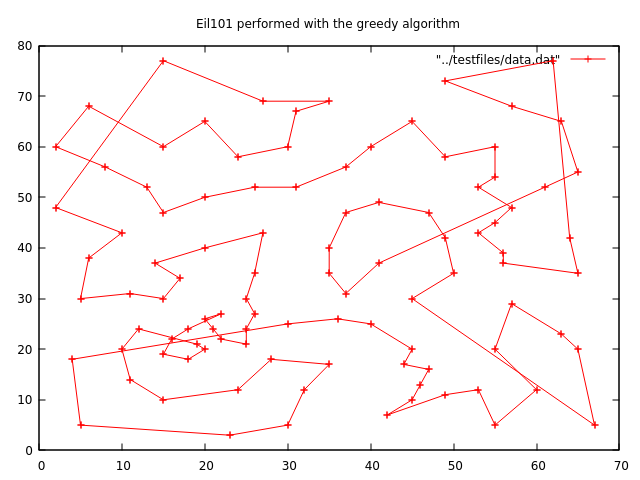
\includegraphics[width=0.6\textwidth]{images/eil101_greedy}
	\caption{In this figure we can see the application to eil101.tsp of the greedy algorithm. In particular we can see the long edges that are chosen since the procedure prefers the nodes that are close to each other.}
\end{figure}

\subsection{Extra-mileage algorithm}
This algorithm is more complex respect to the previous one but in favor of a better solution.

The idea in which the extra-mileage is the following: we start connecting the fartest nodes with both edges (like a cycle), than we search for the closest node to the edges, once it has been identified the edge is substitute with a new couple that insert the the node found in the solution. Let's explain it with the example shown in figure \ref{img:extra}.

\begin{figure}
	\centering
	\begin{subfigure}[b]{0.3\textwidth}
		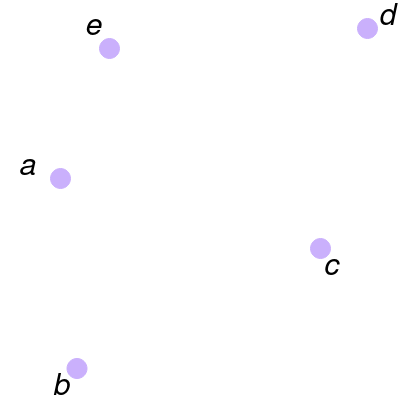
\includegraphics[width=\textwidth]{images/extra_1}
		\caption{No edges}
	\end{subfigure}
	\hfill
	\begin{subfigure}[b]{0.3\textwidth}
		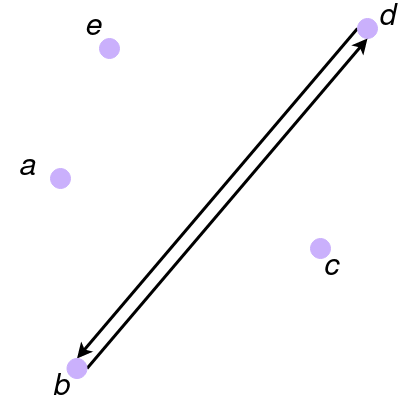
\includegraphics[width=\textwidth]{images/extra_2}
		\caption{First two edges added}
	\end{subfigure}
	\hfill
	\begin{subfigure}[b]{0.3\textwidth}
		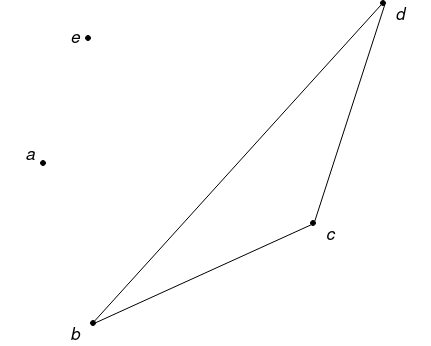
\includegraphics[width=\textwidth]{images/extra_3}
		\caption{One edge is substituted with other two connecting one more node}
	\end{subfigure}
	\bigskip
	\begin{subfigure}{0.3\textwidth}
		\centering
		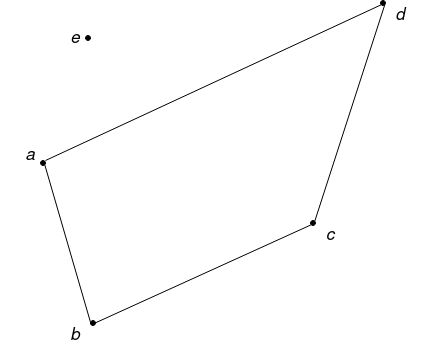
\includegraphics[width=\textwidth]{images/extra_4}
		\caption{Added one more node}
	\end{subfigure}
	\hfill
	\begin{subfigure}{0.3\textwidth}
		\centering
		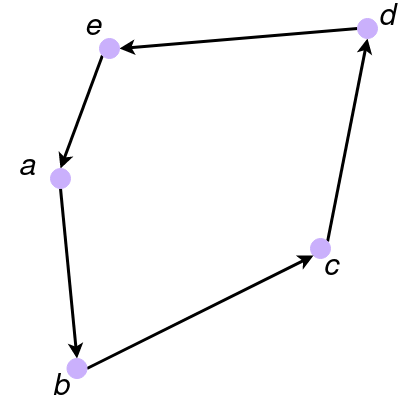
\includegraphics[width=\textwidth]{images/extra_5}
		\caption{All nodes are connected}
	\end{subfigure}
	\caption{In this image we can see the process done by extra-mileage to find the solution.}
	\label{img:extra}
\end{figure}

We start connecting with a cycle the fartest nodes (in this case $c$ and $d$), than we search the node that is closest to theese edges ($c$), once is found we substitute the edge with two more that allow the new node to enter the solution (in this case in order to allow $c$ to enter the solution one of the edges that connect $b$ and $c$ is removed and the edge $x_{bc}$ and $x_{cd}$ are added). This process is repeated until the solution is formed.

We can see the result of the algorithm in figure \ref{img:extra_sol}. Respect to the greedy algorithm we can see that is more ordered with less crossed edges.

\begin{figure}
	\centering
	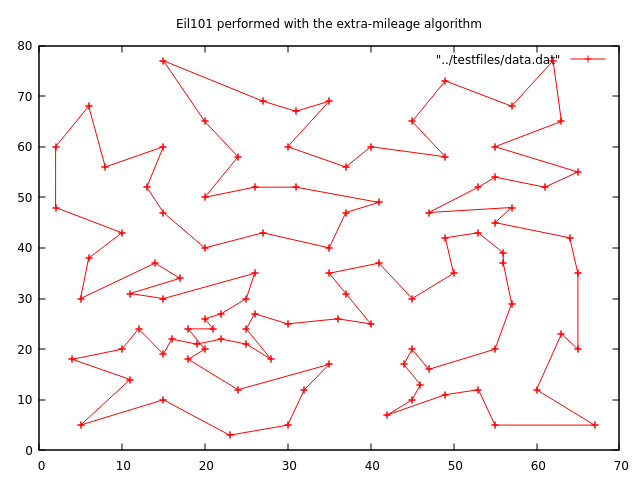
\includegraphics[width=0.6\textwidth]{images/eil101_extra_mileage}
	\caption{In this figure we can see the result of the application of the extra-mileage algortihm to eil101.tsp}
	\label{img:extra_sol}
\end{figure}